\documentclass{article}
\usepackage{graphicx}
\usepackage[top=.5in,bottom=.5in,right=.5in,left=.5in]{geometry}
%\graphicspath{{./../}}
\usepackage{hyperref}
\begin{document}
\title{HERA 10km Fiber tests}
\author{Zuhra Abdurashidova and Jack Hickish}
\maketitle

\section*{Introduction}
This document describes the tests carried out to determine the quality of the 10km fiber optic cable that will be used in the deployment of Hydrogen Epoch of Reionization Array(HERA) in South Africa. Various attenuations and setups were implemented in order to approximate the setup in South Africa. HERA will have various nodes where a collection of SNAP boards will digitize the analog signal coming from the dishes and send it along the fiber optic cable to the correlator approximately 10km away. The use of fiber-optic pluggable transceivers and Mux/Demux pairs will greatly reduce the amount of cables in the system since they combine multiple signals into a single cable. 
\section*{The Basics}
There are probably certain aspects of these experiments that the interested reader is not quiet familiar with. This section will contain some basic definitions.
\begin{itemize}
\item Transceiver-A transceiver in this case is any network device that can both receive and transmit a signal. Transceivers come in different shapes and sizes and the choice for this experiment were the CSFP-10Gb transceivers that support 1270nm, 1290nm, 1310m and 1330nm wavelengths. CSFP stands for Coarse Small Form-factor Pluggable transceiver. Transceivers are wideband and thus could receive any wavelength between 1260nm and 1620nm. However, each transceiver transmits only on the specified wavelength.
\item Multiplexer - Multiplexers these days can both mux and demux a signal. A Mux/Demux pair is a passive device and does not require an external power supply. We used the CWDM(Coarse Wave Division Multiplexer) Mux/Demux pair. The CWDM can both combine(mux) four different laser wavelengths into a COM(common)output and separate(demux)them back to the input wavelengths.  There's a minimal cross talk between the signals in the COM wire since different wavelengths travel at different speeds in a medium. 
\item Attenuator - The intesity of a signal decreases the longer it travels. This is caused by the scattering of light due to imprefections in the fiber, conversion of some of its energy into heat, and absorption. In order to model this type of atenuation in the field, we introduced a few 3dB LC Adapter-type Attenuators and a variable attenuator.
\item Long Distance Network Simulation Test Box(LDNSTB) - This component of the signal chain is essentially a 10km spool of fiber optic cable. It provides an attenuation of about 5.6dB. We managed to successfully add 5dB of attenuation into the system without any data loss - which translates to about 10 additional kilometers of fiber.
\item LC connector - The type of connector used in the fiber optic cables. LC to SC cable was used to connect to the LDNSTB, LC to FC was used to connect to the variable attenuator. Transceivers already come with LC connectors. 
\item Adapters - LC Adapters were used to connect various patches of LC cables(i.e. Mux/Demux to LDNSTB, transceiver LC to Mux/Demux etc). This was necessary since LC connectors all come with a male tip. 
\end{itemize}

\section*{Software}
The boffile was loaded on raspberry pi attached to SNAP board via the python script:
\newline
python sfp\_test.py -b sfp2x\_test\_2015-6-30\_1458.bof -n 2 rpirachel -P 1000 -T 1100
\newline
Each data collection was executed at a wait period of 1100 clock cycles between packet transmissions(-T option). Since SNAP is running at 100MHz, the time between packet transmission is 1100/100e6 = 11 microseconds. The payload of each packet was specified to be 1000, which works out to be 8Kbytes since it is mesured in 64 bit words(-P option). -n option selects the number of cores to be used on SNAP. More information could be found by running python -h sfp\_test.py command. The python script along with other files could be found on github: \url{https://github.com/reeveress/fiber-tests}.

%***************paste github code right heah***************
\section*{Instrument Attenuations}

It is worthwhile to log the attenuations of various instruments involved. The power meter produces a 1310nm, 1KHz wave at -6.50dBm. 
\begin{center}
\begin{tabular}{|l|l|l|l|l|p{2cm}|}
	\hline
	Instrument & Attenuation & Optical Source & Power Meter reading\\ \hline
	Variable attenuator & 3.6dB & -6.50dBm & -10.13dBm\\ \hline
	LDNSTB & 5.6dB & -6.50dBm & -12.10dBm \\ \hline
	Mux/Demux(S/N:92051975) & 1.6dB & -6.50dBm & -8.14dBm \\ \hline
	Mux/Demux(S/N:92051976 & 2.18dB & -6.50dBm & -8.69dBm \\ \hline
	Mux/Demux(1270nm input, COM output) & 33.25dB & -6.50dBm & -39.75dBm \\\hline
\end{tabular}	
\end{center}

\section*{Instrument Overview}
\begin{figure}[h!]
\centering
	\begin{minipage}{.4\textwidth}
		\centering
		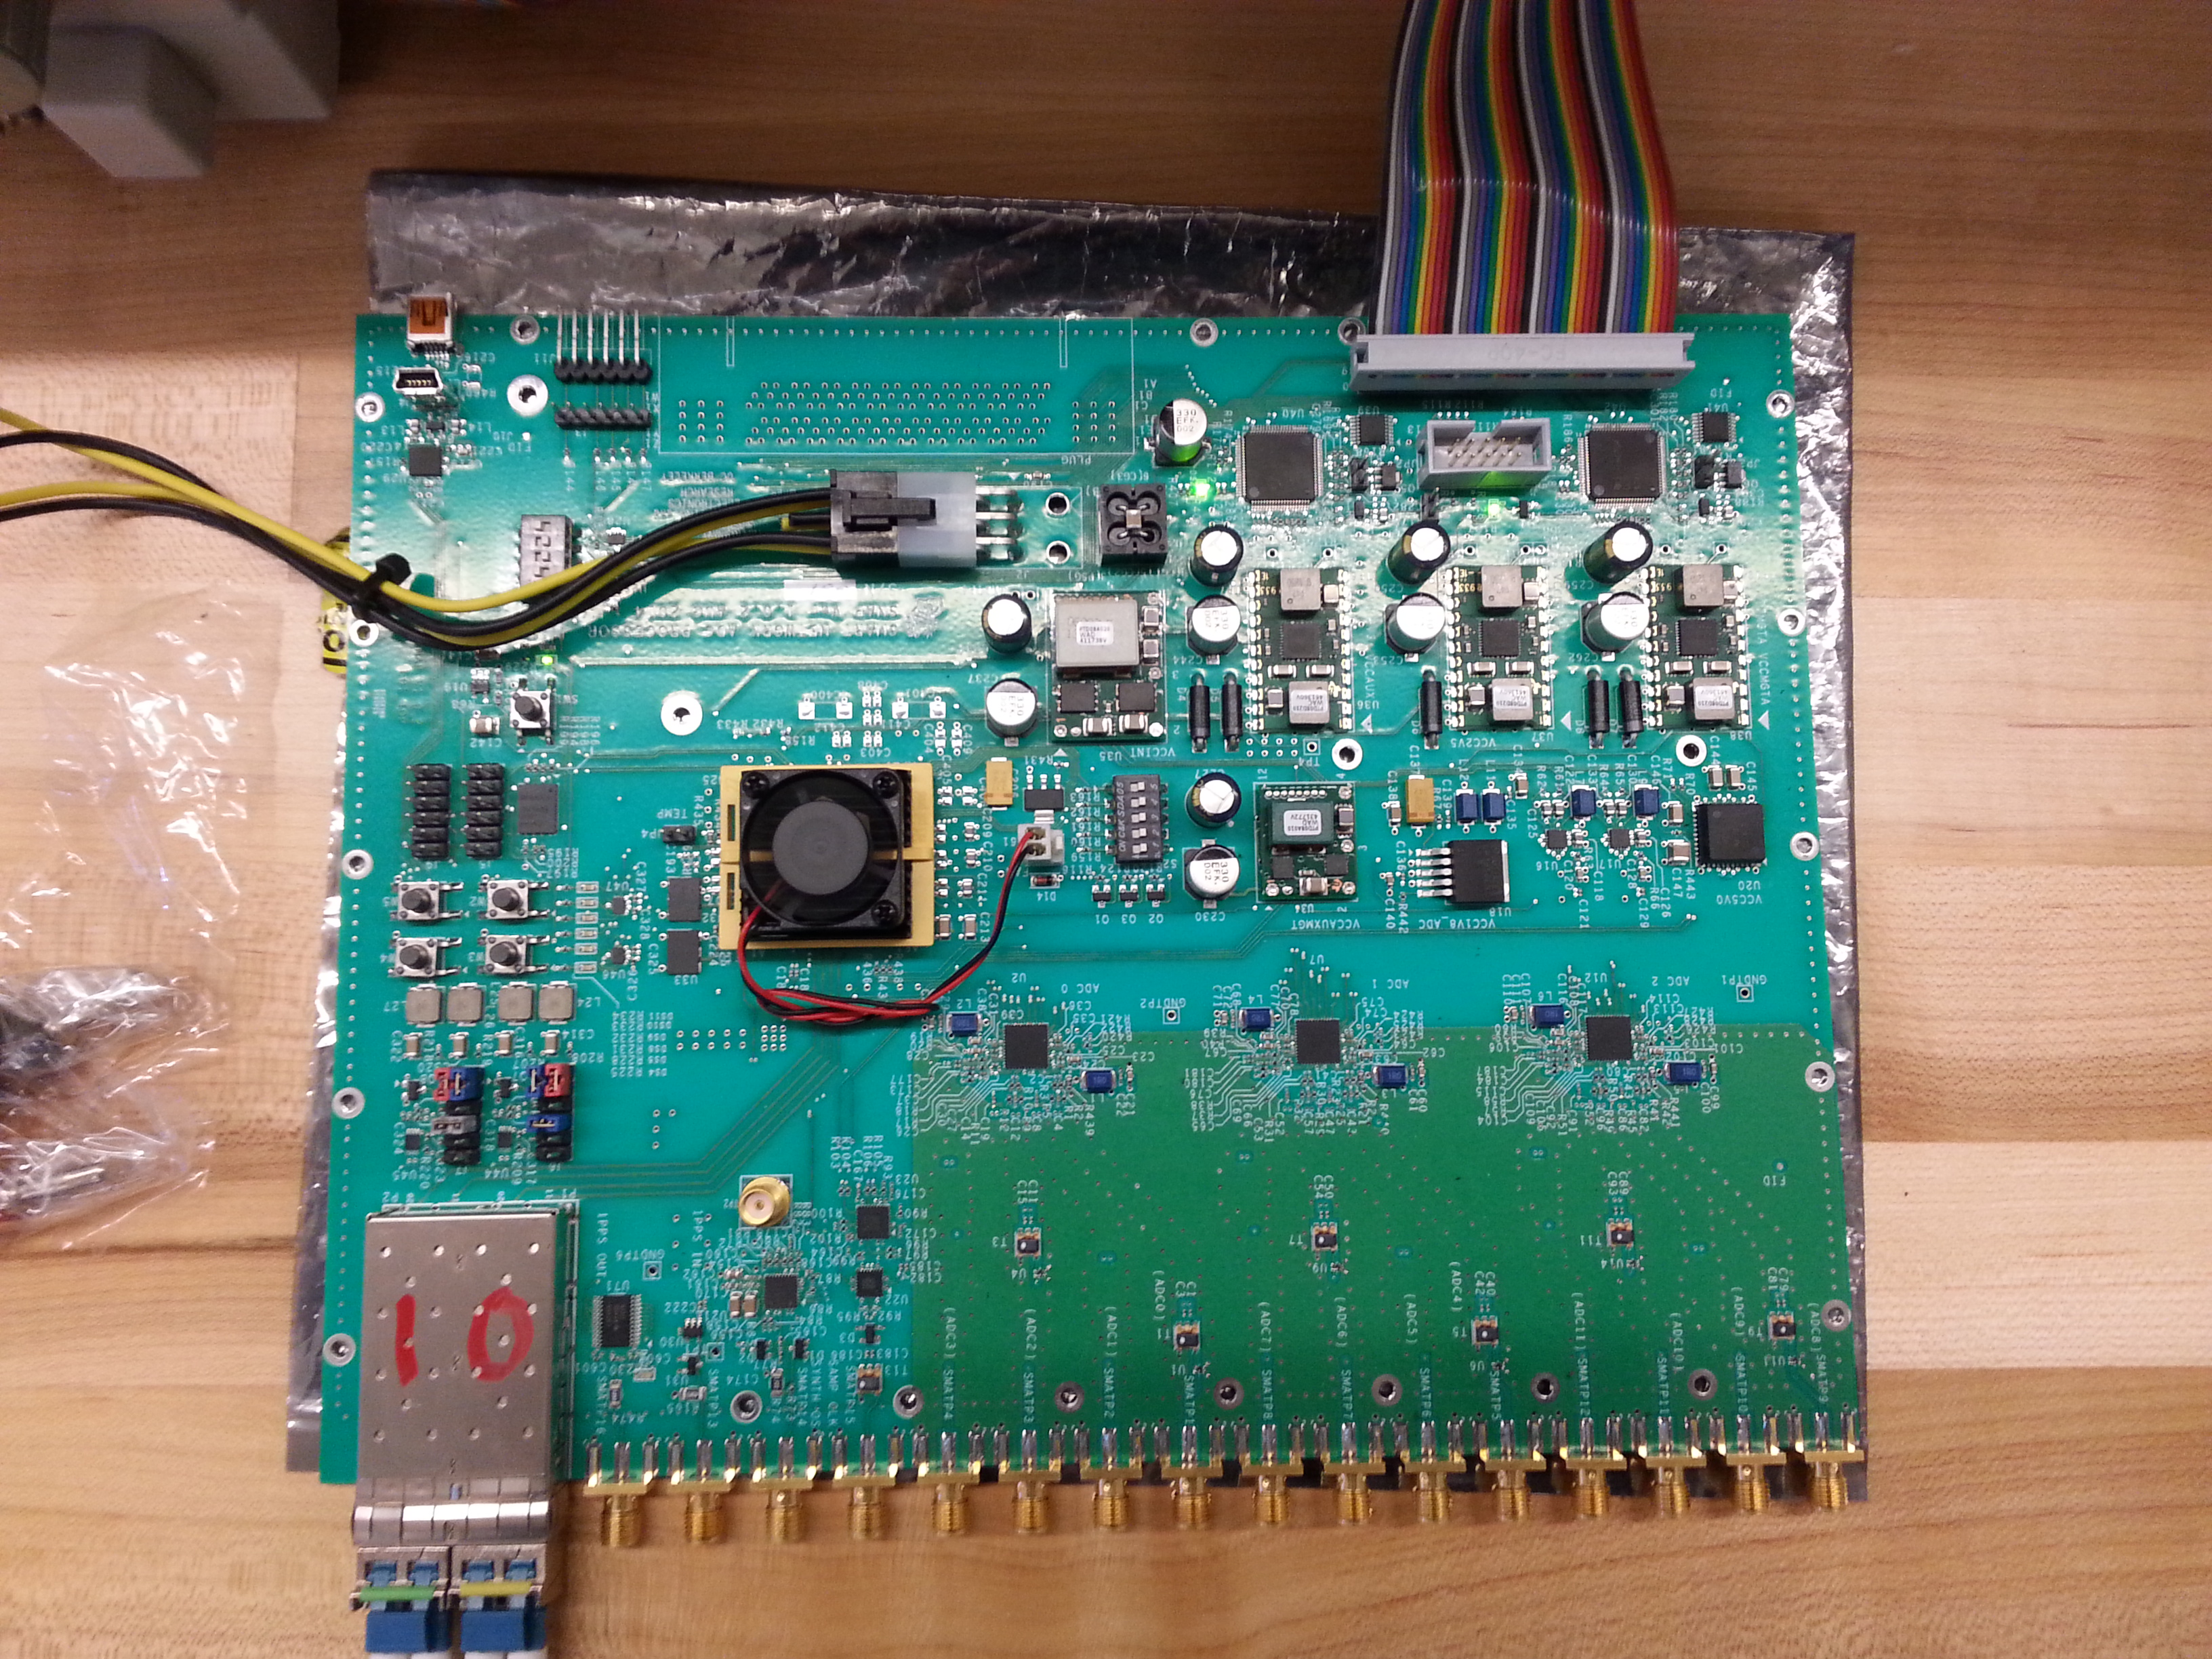
\includegraphics[width =.8\linewidth,height=2.6in]{SNAP.png}
		\caption{SNAP board of S/N: 001} 
	\end{minipage}
	\begin{minipage}{.4\textwidth}
		\centering
		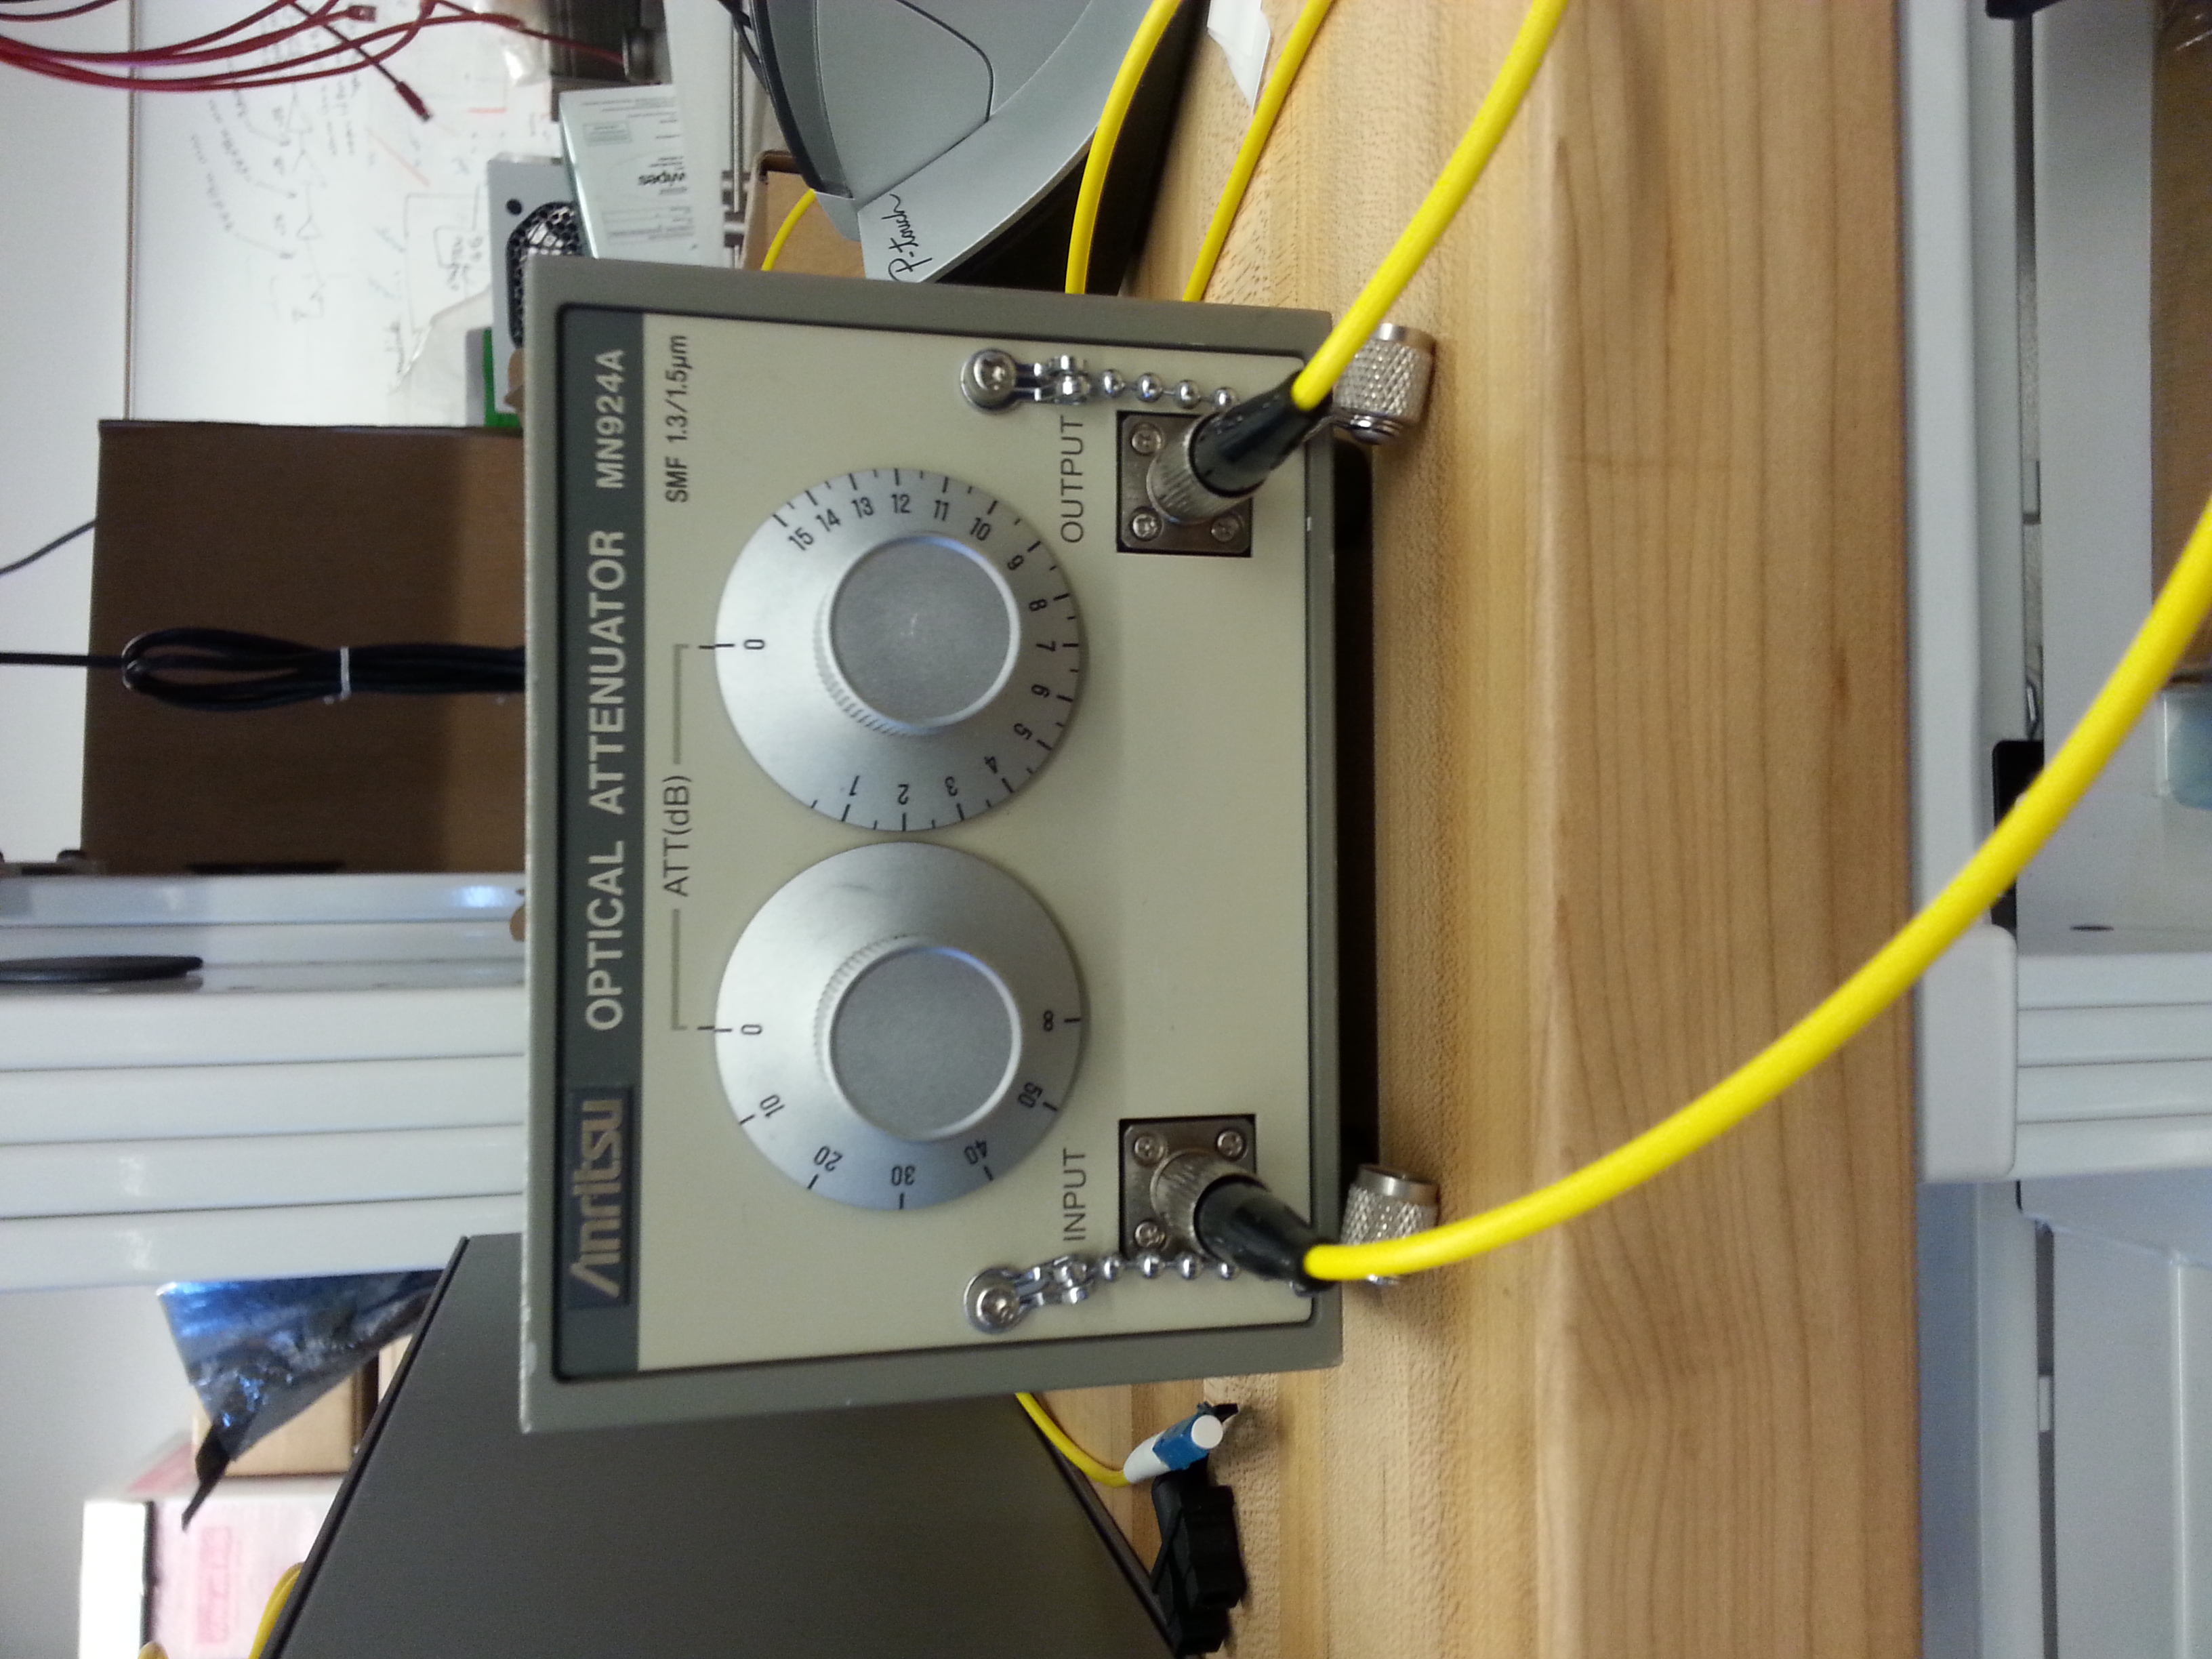
\includegraphics[width = .8\linewidth,height=2.6in]{att.png}
		\caption{Optical Attenuator}
	\end{minipage}
\end{figure}

\begin{figure}[h!]
\centering
	\begin{minipage}{.4\textwidth}
		\centering
		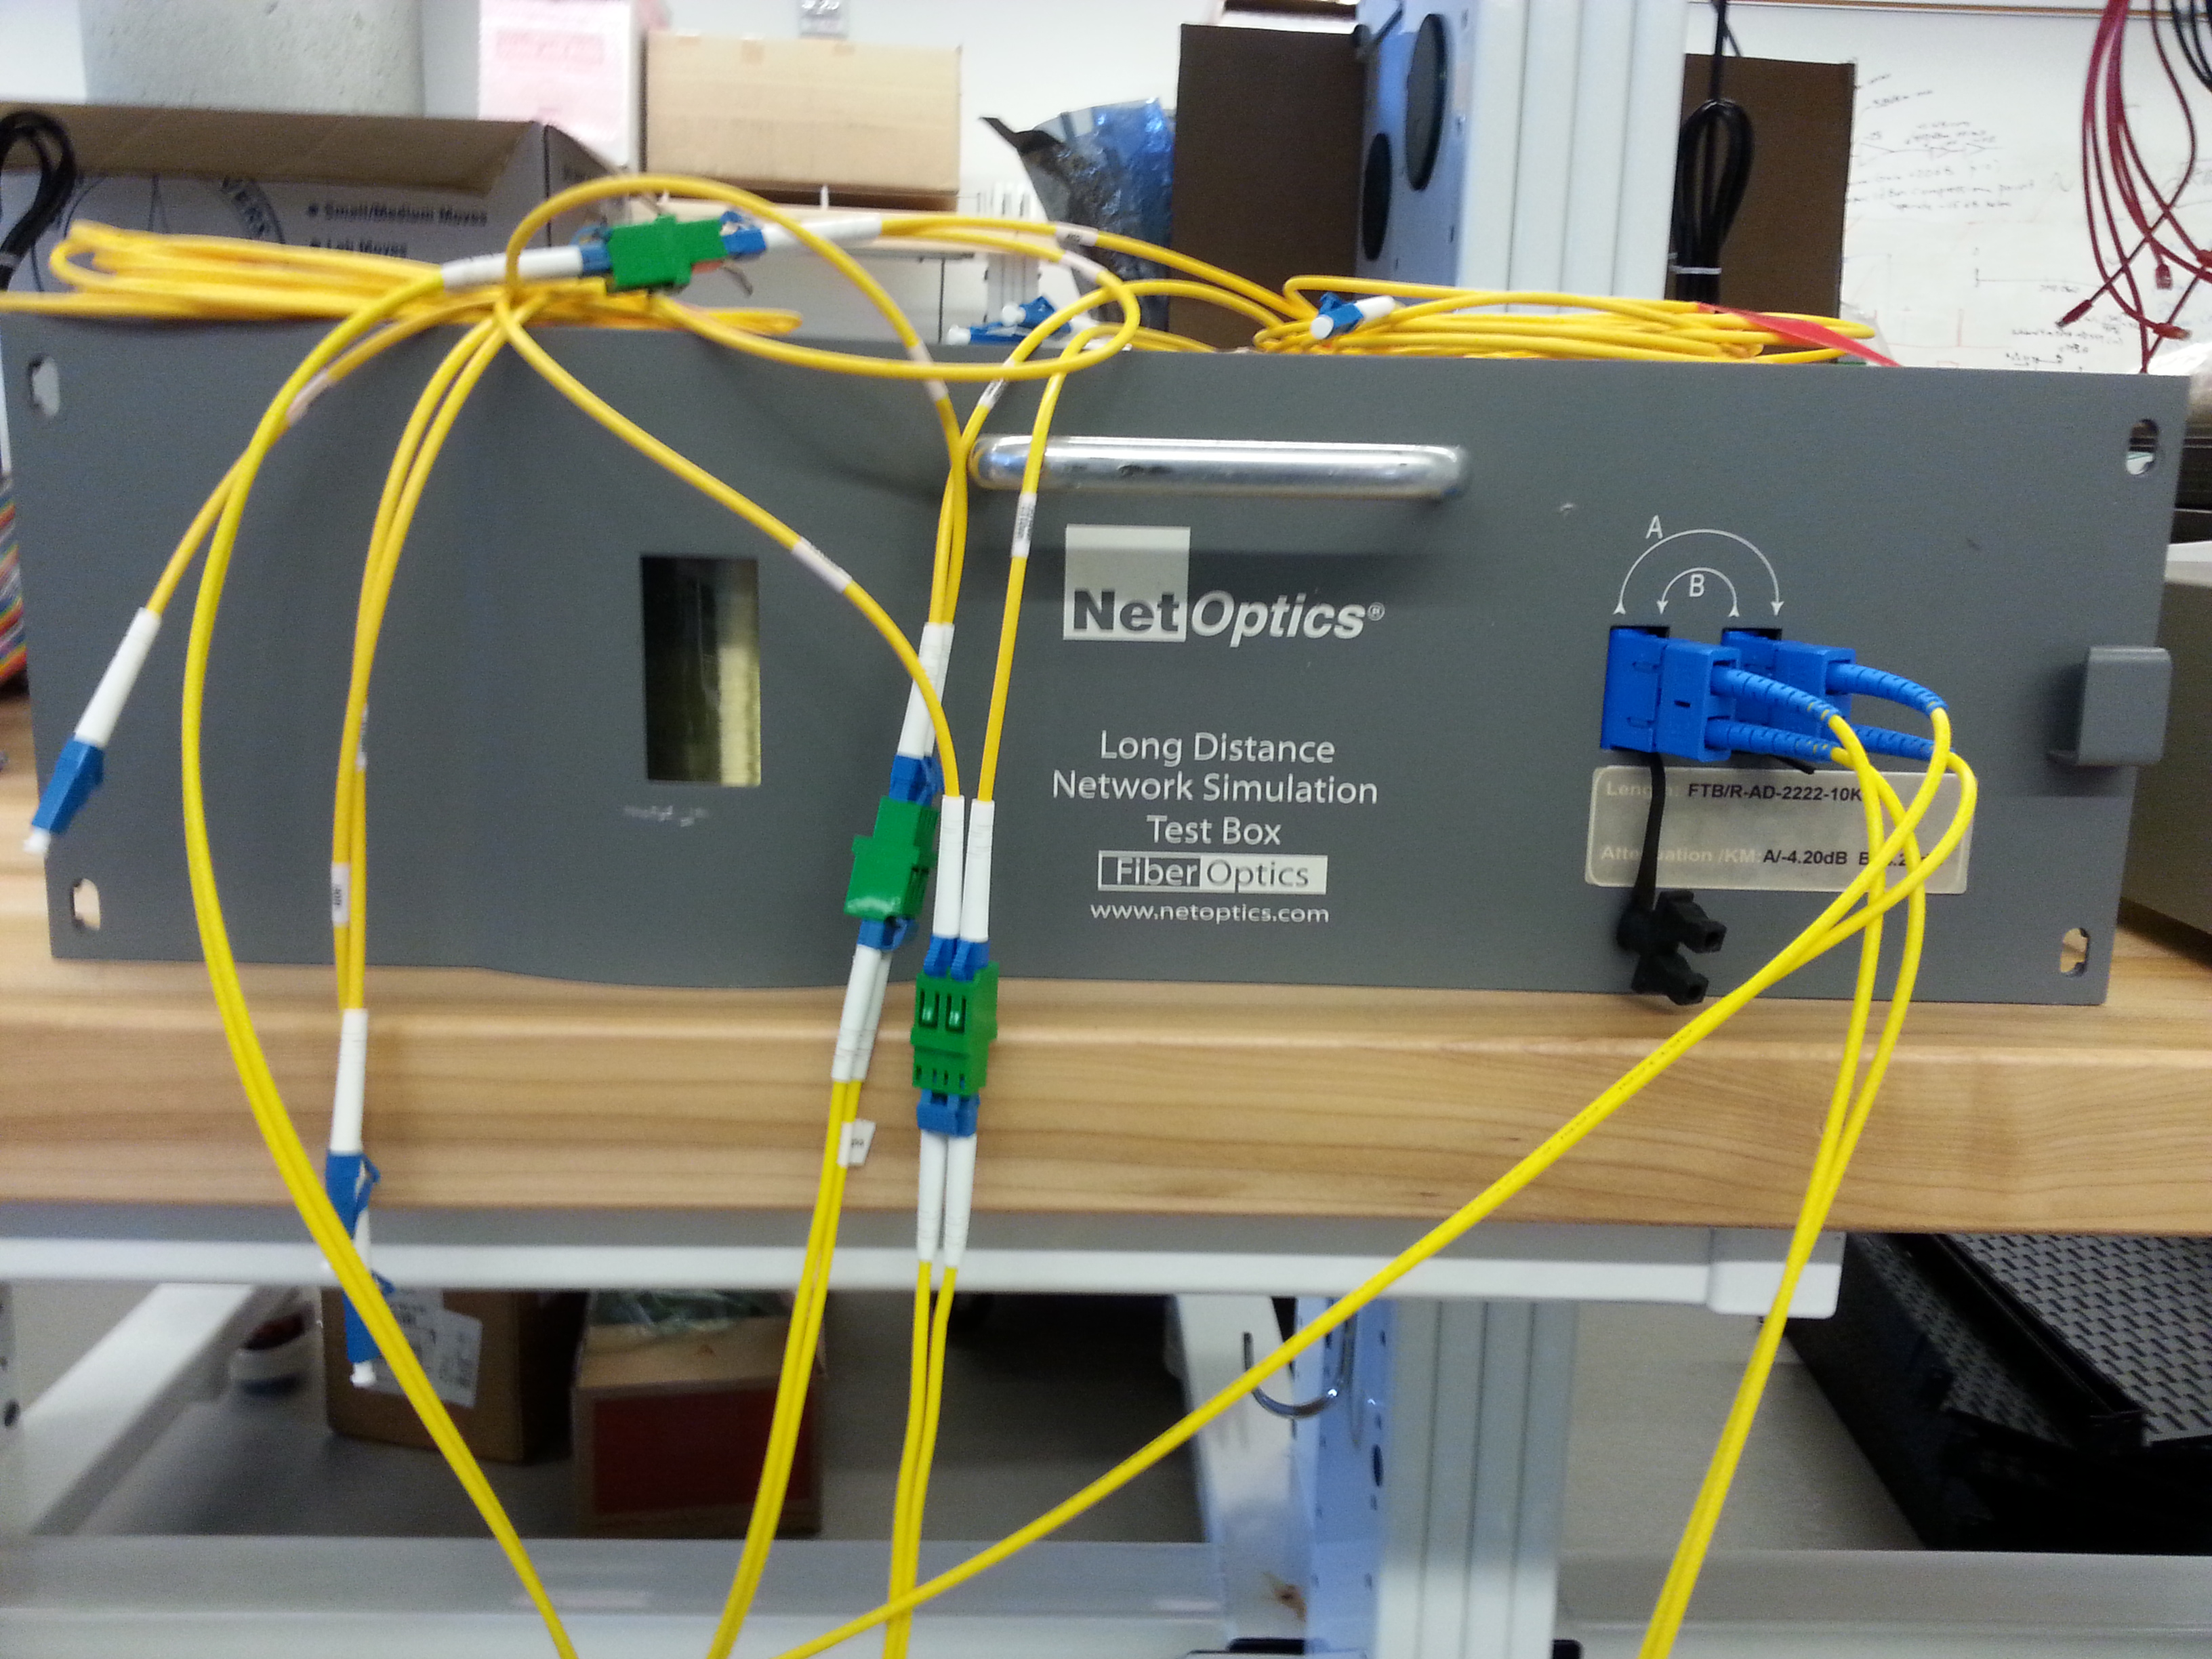
\includegraphics[width = .8\linewidth]{LDNSTB.png}
		\caption{Long Distance Network Simulation Test Box}
	\end{minipage}
	\begin{minipage}{.4\textwidth}
		\centering
		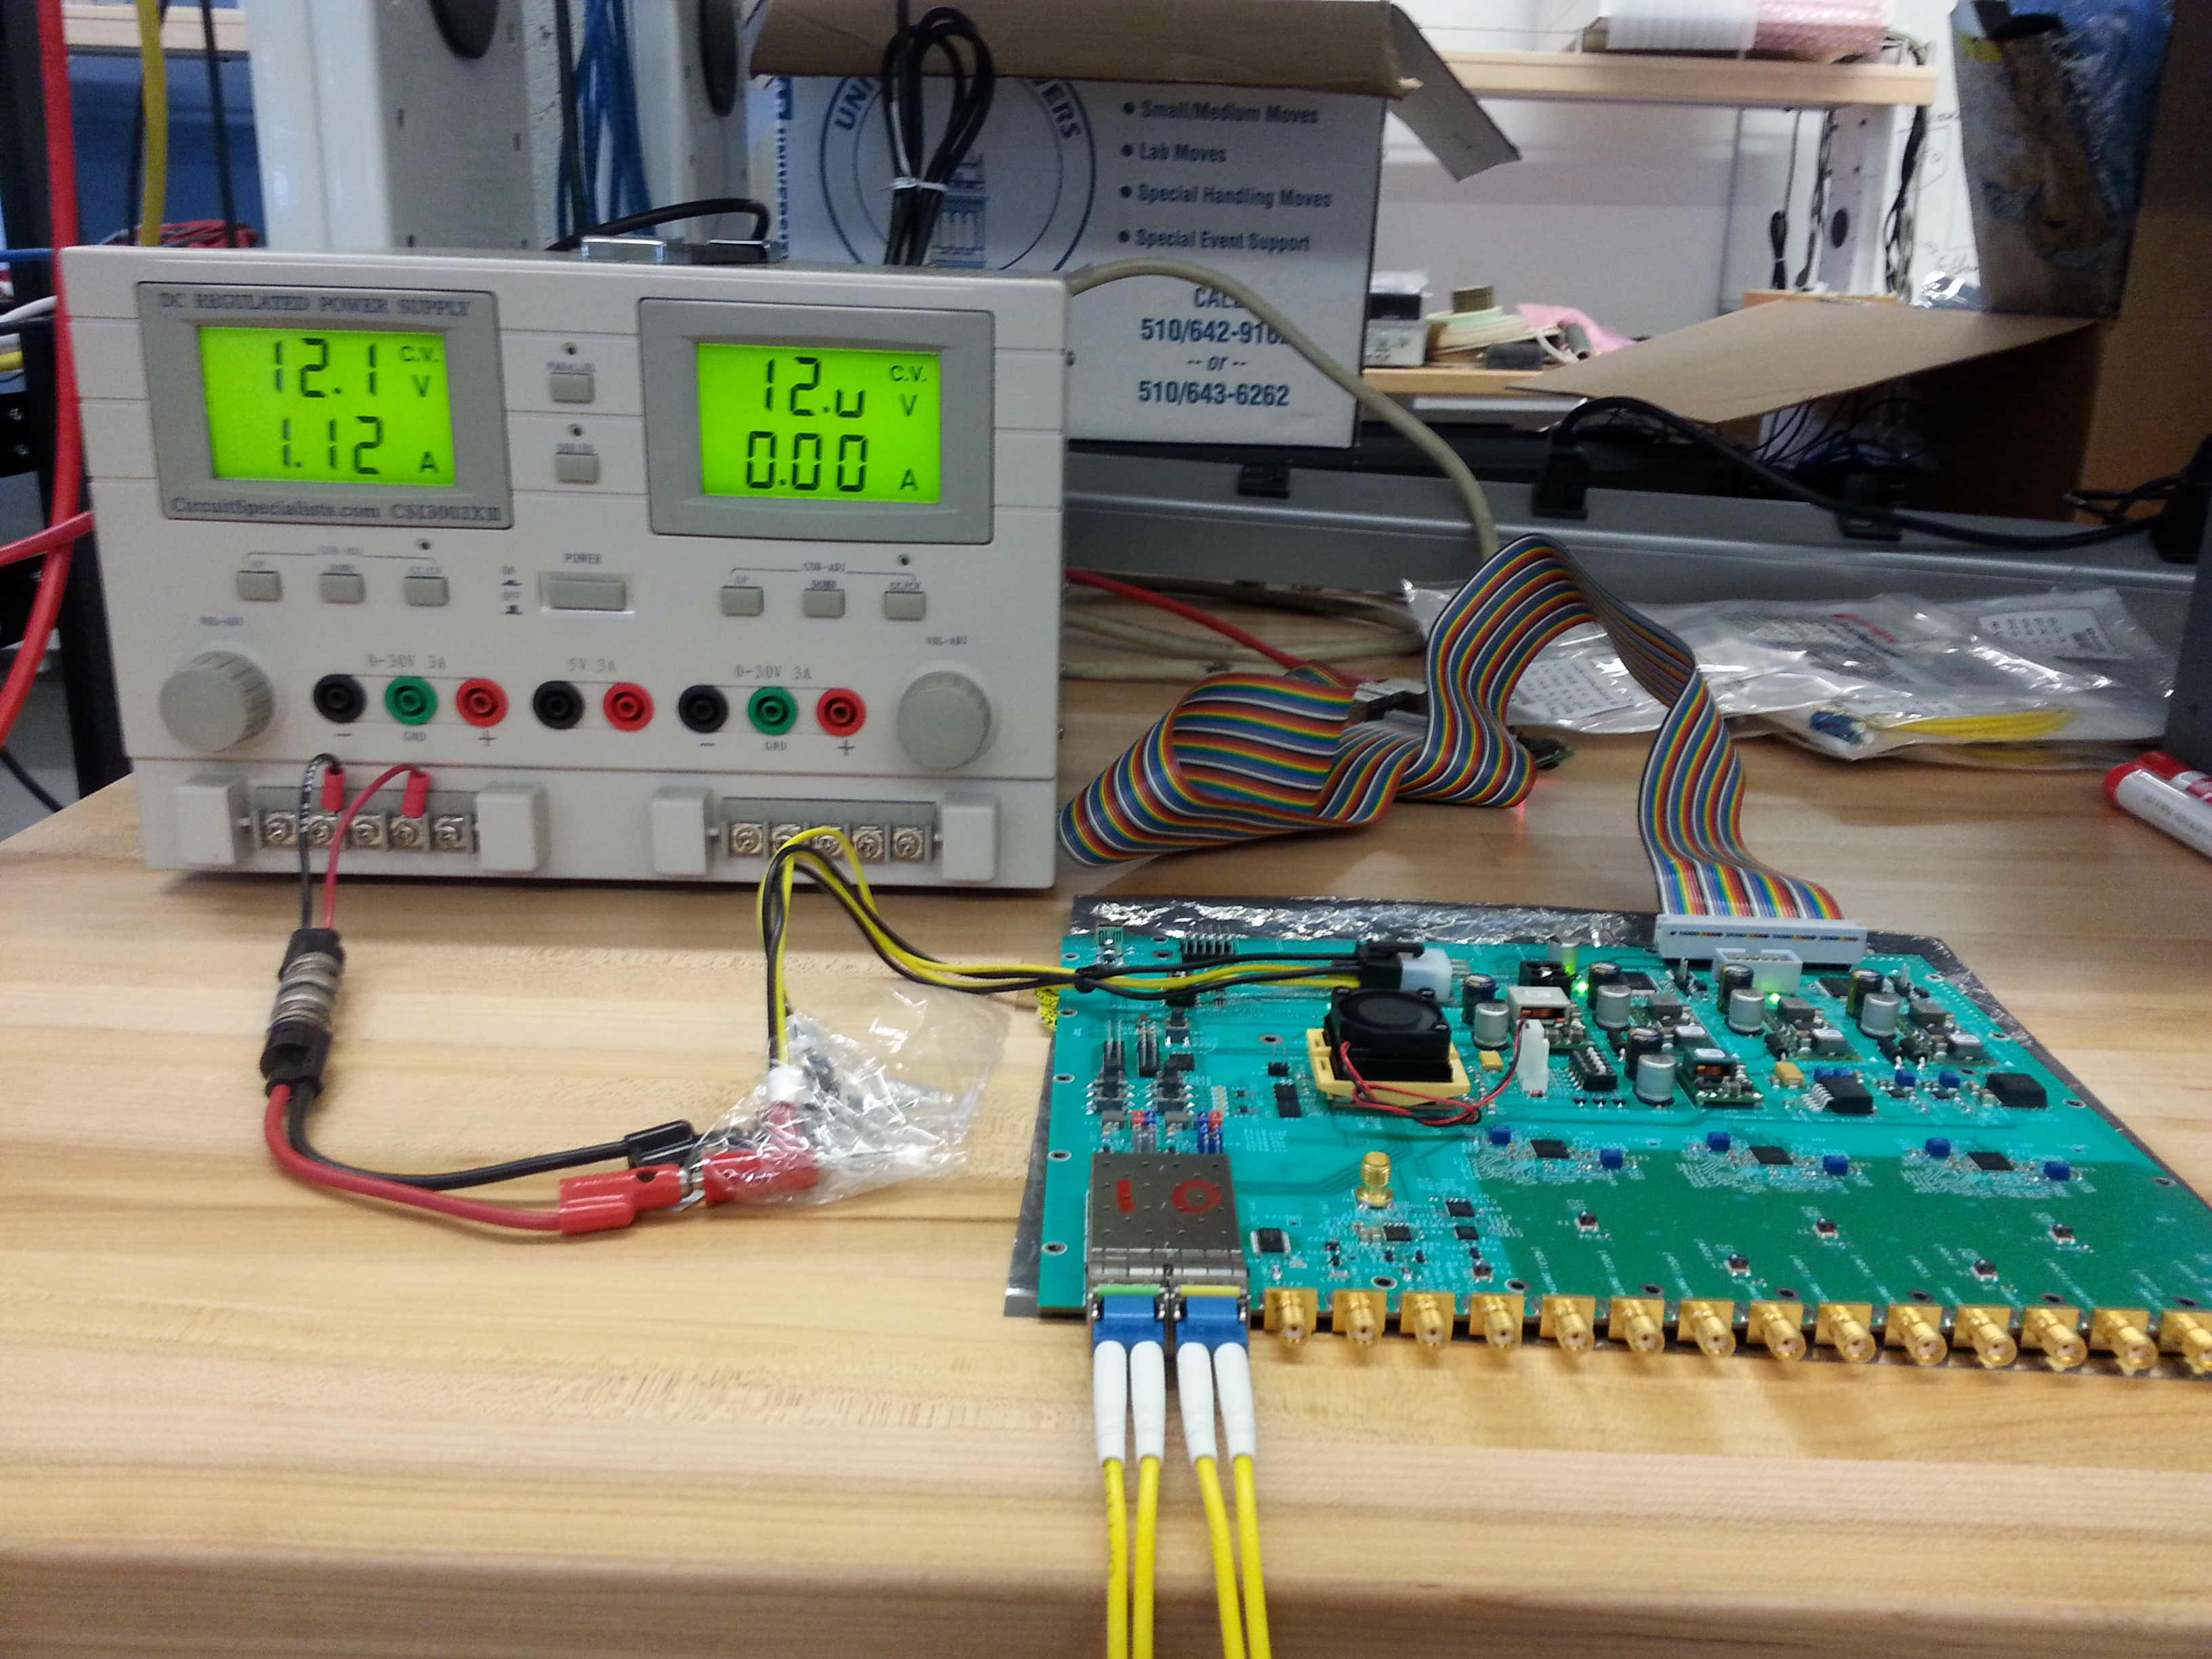
\includegraphics[width = .8\linewidth]{PowerSupply.png}
		\caption{Power Supply for SNAP board}
	\end{minipage}
\end{figure}

\begin{figure}[h!]
\centering
	\begin{minipage}{.4\textwidth}
		\centering
		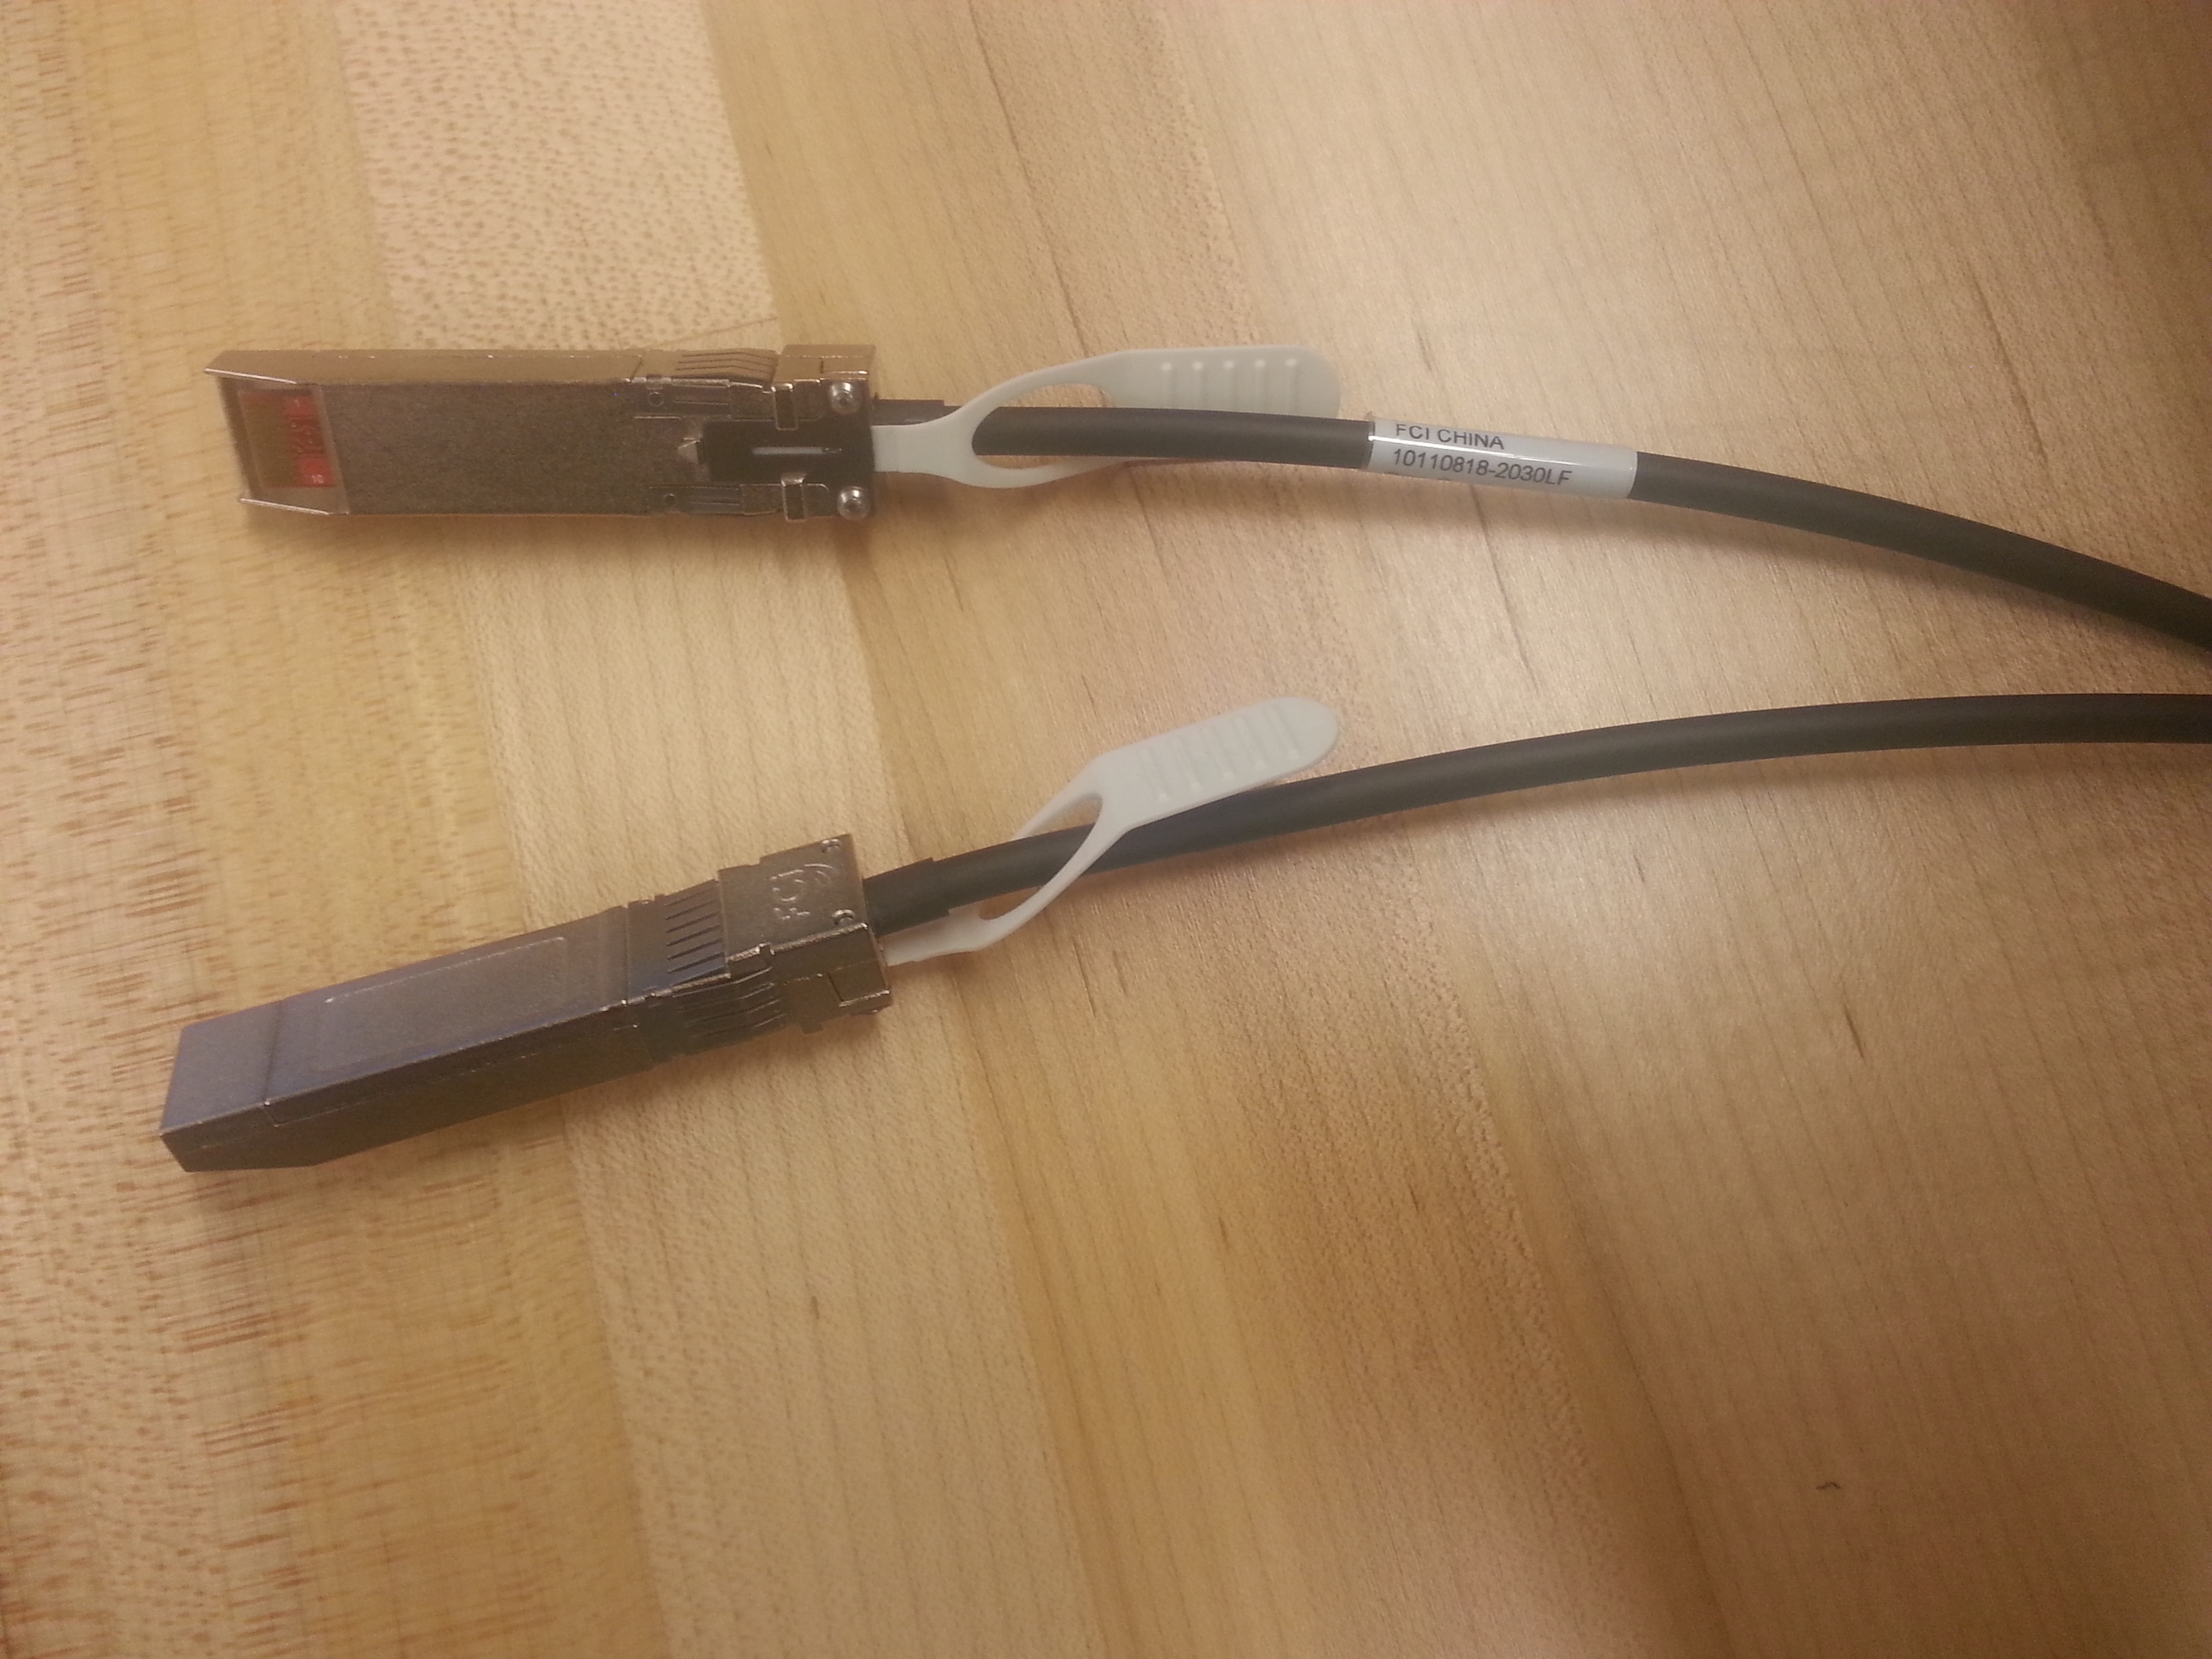
\includegraphics[width = .8\linewidth]{SFPplus.png}
		\caption{3 meter SFP plus copper cable}
	\end{minipage}
	\begin{minipage}{.4\textwidth}
		\centering
		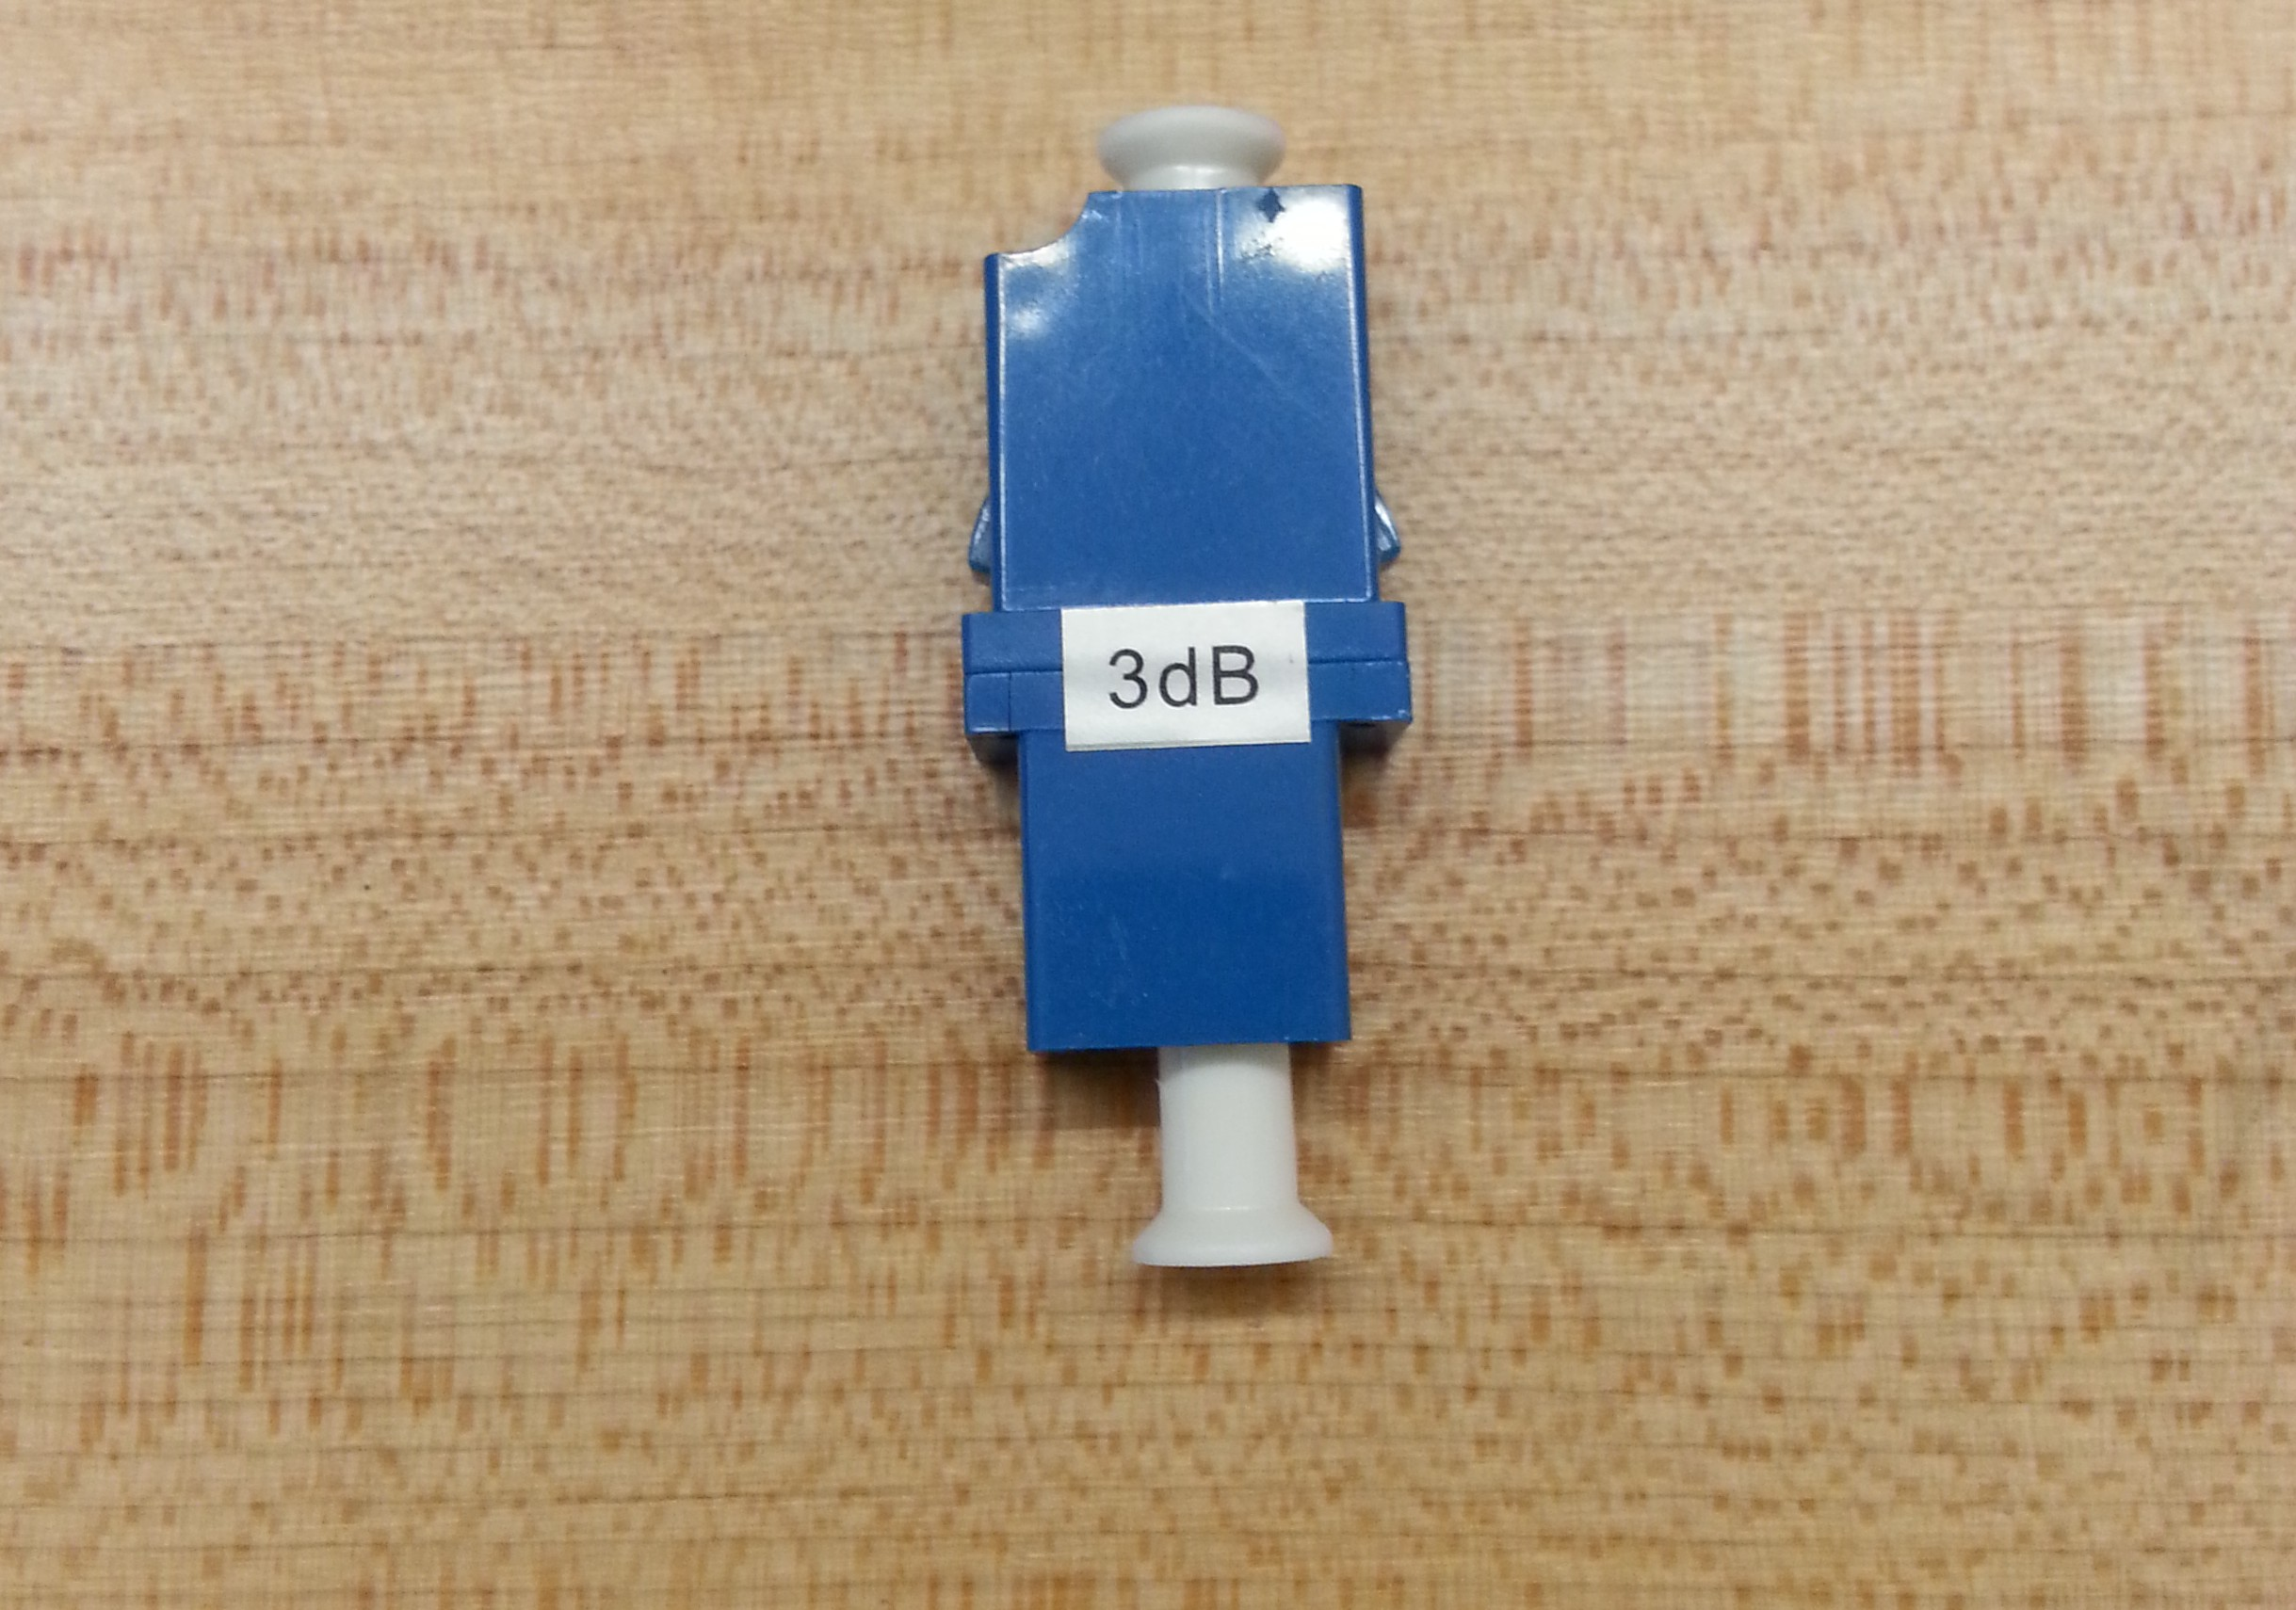
\includegraphics[width = .8\linewidth]{3db.png}
		\caption{3dB Attenuators}
	\end{minipage}
\end{figure}




\section*{Single path Experiment}

The signal is sent from the tx of blue tranceiver on SNAP board's channel 1 and into the left channel of the 10km Long Distance Network Simulation Test Box(LDNSTB). The output came out on the right channel of LDNSTB and into the input of optical attenuator and was routed back into the RX of the red tranceiver on the SNAP board's channel 0. Note that the tx of the red tranceiver(and thus the rx of the blue tranceiver) was not utilized since the variable attenuator we used can only handle a single LC cable input. The attenuation threshold for this setup was found to be around 8dB. Note that such a high attenuation was reached because no mux/demuxes were used, which themselves introduce attenuation into the signal chain. 
The logged data for various attenuations is summarized in the following table:
\begin{center}
\begin{tabular}{|l|l|l|l|p{2cm}|}
	\hline
	Attenuation & Duration & Bytes Transmitted & Packets lost & Bad crcs \\ \hline
	5dB & 46s & 270Mbytes & 0 & 0 \\ \hline
	6dB & 54s & 319Mbytes & 0 & 0 \\ \hline
	7dB & 70s & 410Mbytes & 0 & 0 \\ \hline
	8dB & 64s & 374Mbytes & 1 & 5 \\ \hline
	9dB & 87s & 508Mbytes & 5 & 912 \\ \hline
	10dB & 62s & 361Mbytes & 5648464 & 0 \\ \hline 
	
\end{tabular}
\end{center}

\begin{figure}[h!]
	\centering
	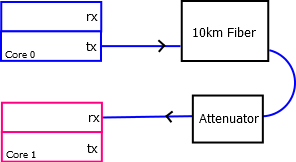
\includegraphics[width = .6\linewidth]{singlepath080415.png}
	\caption{Signal Flow Diaram for Single Path Experiment}
\end{figure}


\section*{Double Path Experiment}
In order to test attenuation in both directions we used the two 3dB attenuators and wired it into the circuit as shown in Figure~\ref{fig:doublefiber}. Both cores transmitted without lost or corrupt packets. 

\begin{figure}[h!]
\centering
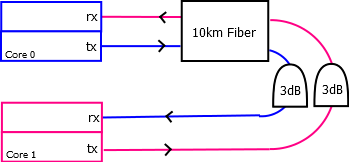
\includegraphics[width=.5\textwidth]{doublepath080415.png}
\caption{Double Path Diagram}
\label{fig:doublefiber}
\end{figure}







\section*{Demux experiment}
The output of the blue transceiver at the SNAP's core 0 was connected through an LC adapter to the 1290nm cable of Mux/Demux(S/N:92051975). Similarly, the output of the pink transceiver at core 1 was connected to the 1270nm cable of the same Mux/Demux. The muxed COM cable was then connected through an LC adapter to the bottom input of the LDNSTB left channel. The output was taken from the top output of the LDNSTB right channel and routed into the COM cable of the Mux/Demux of S/N:92051976. This Mux/Demux then split the COM signal into the respective wavelengths. The 1290nm(blue)signal was send into the pink transceiver and 1270nm(pink)signal was send into the input of the blue transceiver. To prevent packet loss, it is necessary to send signals of a certain wavelength to a transceiver of a different wavelength. This prevents the cross-talk between the signals that causes data corruption. Summary of the test:
\begin{center}
\\
\begin{tabular}{|l|l|l|l|p{2cm}|}
	\hline
	Attenuation & Duration & Bytes Transmitted & Packets lost & Bad crcs \\ \hline
	0dB & 4142s & 3 TeraBytes & 0 & 0 \\ \hline
\end{tabular}	
\end{center}
%insert a snap of test results and repeat the test with 6db connected to the setup  

\section*{Demux/switch experiment}
To better emulate the actual signal flow at HERA, we wired up a switch into our existing setup(Figure~\ref{fig:demuxdiag}). The signals were sent from the pink transceiver tx at Core 1 and blue tranceiver tx at Core 0. The tx of pink transceiver was connected through LC adapter and LC/FC cable to the variable attenuator's input, the output was connected through FC/LC cable and LC adapter to the 1270nm cable of left mux/demux. Blue tx is connected through LC cable to the 1290nm cable of the left mux/demux(S/N:92051975). The COM of that mux/demux was connected to the bottom input of the left channel of LDNSTB, the output of LDNSTB(upper pin of the right channel)was connected through SC to LC cable and LC adapter to the right mux/demux(S/N: 92051976). The demuxed 1290nm line is connected via the two LC cable and two LC adapters(cascaded for extension)to the yellow 1330nm transceiver at the switch. Similarly, the 1270nm demuxed line is connected to the green(1310nm) transceiver at the switch. The tx of the green switch is then routed back to the green(1310nm line of the right mux/demux(S/N: 92051976. Same goes for the tx of the yellow transceiver at the switch. These signals were then muxed and sent through the COM to LDNSTB and back out through SC/LC cable, LC adapter and to the COM of the left mux/demux(S/N 91051975). The signals were then demuxed and routed to the rx's of the transceivers at the SNAP board. 1330nm went to the blue rx and 1310nm signal went to the pink rx. Note: the signals were traveling on the COMs of the two mux/demuxes in both directions. Blue and pink signals are gettig muxed at the left mux/demux and the green/yellow signals are getting demuxed at that same mux/demux. Since the signals are sent to the switch and back again, the signals travel a total of 20km(plus all the LC/FC, LC, LC/SC cables).Note that the switch takes some time to configure so after initial packet loss of about 300,000 no further packet loss/corruption occurs. 
Test Results:
\begin{center}
\begin{tabular}{|l|l|l|l|l|p{2cm}|}
	\hline
	& Attenuation & Duration & Bytes Transmitted & Packets lost & Bad crcs \\ \hline
	Core 0 & 5dB & 8380s & 6.1Gbytes & 0 & 1 \\ \hline
	Core 1 & 5dB & 8380s & 6.1Gbytes & 0 & 1 \\ \hline
\end{tabular}	
\end{center}

\begin{figure}[h!]

	\centering
	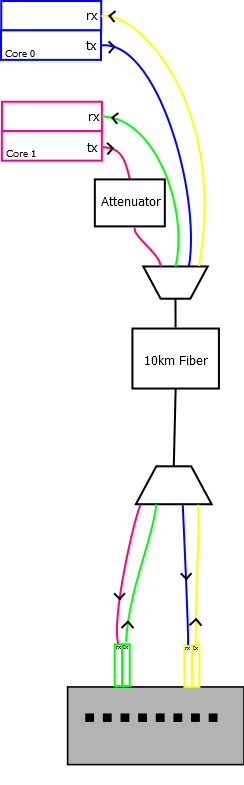
\includegraphics[width=.3\linewidth]{muxswitch080415.png}
	\caption{Signal flow of the Demux/switch experiment}
	\label{fig:demuxdiag}
\end{figure}



\section*{Demux/switch/3m Copper connection}

The final test was designed to see if having a 20km round trip signal distance had a major affect on the attenuation threshold. Thus instead of having two tranceivers on each end of the connection we had one at the SNAP core, one at the switch and  added a 3 meter SFP plus copper cable that connected the switch to one of the cores on the SNAP board, as shown in Figure~\ref{fig:demuxdiagCu}. The signal flow was as follows: Packets are sent from the tx of pink transeiver at the SNAP Core 1 to the variable attenuator, to the left mux/demux, COM to LDNSTB to the COM of right mux/demux, 1270nm LC cable to the switch and back to the SNAP Core 0 via the SFP plus cable. The threshold remained unchanged from the previous setup(~5dB before the onset of catastrophic packet loss). 


%JACK's test:The threshold remained unchanged from the previous setup(~9dB for the onset of catastrophic packet loss).********
\begin{center}
\begin{tabular}{|l|l|l|l|l|p{2cm}|}
	\hline
	& Attenuation & Duration & Bytes Transmitted & Packets lost & Bad crcs \\ \hline
	Core 0 & 5dB & 14597s & 10.6 Gbytes & 0 & 1 \\ \hline
	Core 1 & 5dB & 14597s & 0.17 Gbytes & 0 & 1 \\ \hline
\end{tabular}	
\end{center}


\begin{figure}[h!]
	\centering
	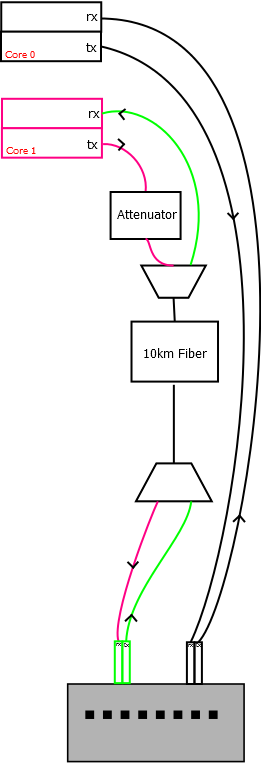
\includegraphics[width = .3\linewidth]{muxswitchcu080415.png}
	\caption{Singal flow of the Demux/switch/Cu wire}
	\label{fig:demuxdiagCu}
\end{figure}

\section*{Conclusion}
These tests show that the 10km of fiber between the HERA dishes and correlator should not impose any problems for data throughput. In addition to the 10km which indtroduce about 5dB of attenuation into the system, we were able to attenuate the signal by additional 7-8dBs since the variable attenuator used produced about 3dBs of attenuation. LC adapters and various LC cable connections should be avoided as they introduce additional attenuation and catastrophic packet loss if connected improperly; splicing should be be used where possible. Switches have a short period of configuration during which packet loss occurs. 
\end{document} 
